\documentclass[a4,11pt]{aleph-notas}
% Se puede ver la documentación aquí: 
% https://github.com/alephsub0/LaTeX_aleph-notas

% -- Paquetes adicionales 
\usepackage{enumitem}
\usepackage{aleph-comandos}
\usepackage{booktabs}
\usepackage[spanish, ruled, vlined, onelanguage]{algorithm2e}

\usepackage{tikz}
\usetikzlibrary{arrows.meta,calc,positioning,decorations.markings}

% -- Datos 
\institucion{Facultad de Ciencias Exactas, Naturales y Ambientales}
\carrera{Ciencia de Datos}
\asignatura{Aprendizaje Automático Inicial}
\tema{Resumen no. 11: Support Vector Machine (SVM)}
\autor{Andrés Merino}
\fecha{Periodo 2025-2}

\logouno[0.14\textwidth]{Logos/logoPUCE_04_ac}
\definecolor{colortext}{HTML}{0030A1}
\definecolor{azul}{HTML}{0030A1}
\definecolor{rojo}{HTML}{A10030}
\definecolor{verde}{HTML}{30A100}
\definecolor{colordef}{HTML}{0030A1}
\fuente{montserrat}


% -- Comandos adicionales
\setlist[enumerate]{label=\roman*.}
\SetAlCapFnt{\normalfont\bfseries}
\SetAlgoCaptionSeparator{\par\nobreak}
\SetAlCapNameFnt{\unskip\itshape}
\SetKwInOut{Input}{Entrada}
\SetKwInOut{Output}{Salida}

\begin{document}

\encabezado


\section*{Support Vector Machine (SVM)}

Vladimir Vapnik dijo: \textit{«No existe nada más práctico que una buena teoría»}.

\begin{defi}
Sea un conjunto de entrenamiento $\left\{({x}_i, y_i)\right\}_{i=1}^N$ donde ${x}_i \in \mathbb{R}^n$ son los vectores de características y $y_i \in \{-1, 1\}$ son las etiquetas de clase.

El modelo SVM busca determinar un hiperplano, definido por $${w} \cdot {x} + b = 0,$$ que separe los datos, es decir
\[
    {w} \cdot {x}_i + b \geq 1\ \text{ si }\ y_i = 1
    \texty
    {w} \cdot {x}_i + b \leq -1\ \text{ si }\ y_i = -1.
\]
\end{defi}

\begin{advertencia}
La condición puede tomarse como:
    $$y_i ({w} \cdot {x}_i + b) \geq 1$$
\end{advertencia}

\begin{advertencia}
A los vectores que alcanzan la igualdad de la condición, es decir, $y_i ({w} \cdot {x}_i + b) = 1$, se los llama \textbf{vectores de soporte}.
\end{advertencia}

\begin{center}
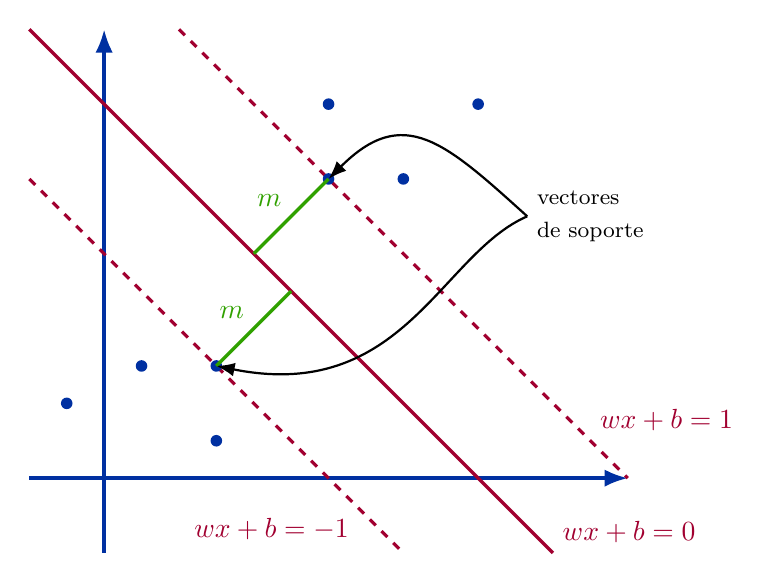
\begin{tikzpicture}[scale=0.95]
    % ---- Fondo tipo cuadrícula ----
    % \draw[step=0.5,very thin,azul!15] (-1,-1) grid (7,6);
    % \draw[step=1,thin,azul!25] (-1,-1) grid (7,6);
    % ---- Ejes ----
    \draw[azul,very thick,-{Latex}] (-1,0) -- (7,0);
    \draw[azul,very thick,-{Latex}] (0,-1) -- (0,6);
    % ---- Rectas (SVM) ----
    \draw[rojo,very thick] 
        plot[domain=-1:6] (\x, {-1*\x + 5});
    \draw[rojo,very thick,dashed] 
        plot[domain=1:7] (\x, {-1*\x + 7});
    \draw[rojo,very thick,dashed] 
        plot[domain=-1:4] (\x, {-1*\x + 3});

    % ---- Etiquetas de rectas ----
    \node[rojo,above right] at (6,-1) {$w x + b = 0$};
    \node[rojo,above right] at (6.5,0.5) {$w x + b = 1$};
    \node[rojo,below left]  at (3.4,-0.4) {$w x + b = -1$};

    % ---- Vectores de soporte (puntos sobre los márgenes) ----
    \coordinate (sv1) at (3,{ -1*(3) + 7});
    \coordinate (sv2) at (1.5,{ -1*(1.5) + 3});

    \fill[azul] (sv1) circle (2.2pt);
    \fill[azul] (3,5) circle (2.2pt);
    \fill[azul] (4,4) circle (2.2pt);
    \fill[azul] (5,5) circle (2.2pt);
    \fill[azul] (sv2) circle (2.2pt);
    \fill[azul] (-0.5,1) circle (2.2pt);
    \fill[azul] (0.5,1.5) circle (2.2pt);
    \fill[azul] (1.5,0.5) circle (2.2pt);

    % ---- Segmento / vector t (verde) ----
    \draw[verde,very thick,-] (sv1) -- (2,3);
    \draw[verde,very thick,-] (sv2) -- (2.5,2.5);
    \node[verde,above left] at ($(sv1)!0.5!(2,3)$) {$m$};
    \node[verde,above left] at ($(sv2)!0.5!(2.5,2.5)$) {$m$};

    % ---- Etiquetas: vectores de soporte ----
    \node[black,align=left] (lab1) at (6.5,3.5) {\footnotesize vectores\\\footnotesize de soporte};
    \draw[-{Latex},black,thick] (lab1.west) .. controls (4.55,4.5) and (4,5) .. (sv1);
    \draw[-{Latex},black,thick] (lab1.west) .. controls (4.5,3) and (4,1) .. (sv2);

\end{tikzpicture}
\end{center}


La distancia de los vectores de soporte al hiperplano separador es $m$ (margen). El objetivo es maximizar el margen, que es la distancia entre los hiperplanos por los que pasan los vectores de soporte: $2m$.  

Para determinar el valor de $t$, consideremos momentáneamente que el hiperplano pasa por el origen (es decir, $b=0$).
\begin{center}
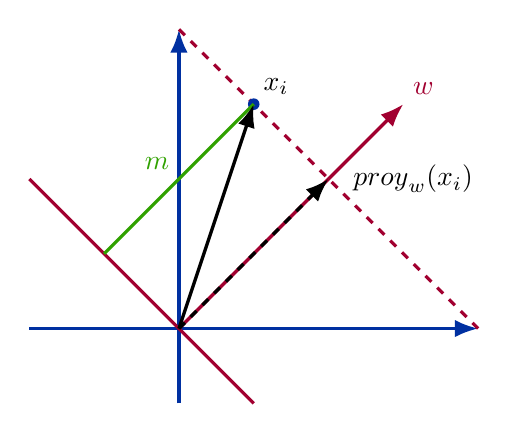
\begin{tikzpicture}[scale=0.95]
    % ---- Fondo tipo cuadrícula ----
    % \draw[step=0.5,very thin,azul!15] (1,1) grid (7,6);
    % \draw[step=1,thin,azul!25] (1,1) grid (7,6);
    % ---- Ejes ----
    \draw[azul,very thick,-{Latex}] (1,2) -- (7,2);
    \draw[azul,very thick,-{Latex}] (3,1) -- (3,6);
    % ---- Rectas (SVM) ----
    \draw[rojo,very thick] 
        plot[domain=1:4] (\x, {-1*\x + 5});
    \draw[rojo,very thick,dashed] 
        plot[domain=3:7] (\x, {-1*\x + 9});

    % ---- Vectores de soporte (puntos sobre los márgenes) ----
    \coordinate (sv1) at (4,{ -1*(4) + 9});
    \fill[azul] (sv1) circle (2.2pt);

    % ---- Segmento / vector t (verde) ----
    \draw[verde,very thick,-] (sv1) -- (2,3);
    \node[verde,above left] at ($(sv1)!0.5!(2,3)$) {$m$};

    \draw[rojo,very thick,-{Latex}] (3,2) -- (6,5);
    \node[rojo,above right] at (6,5) {$w$};

    \draw[very thick,-{Latex}] (3,2) -- (4,{ -1*(4) + 9});
    \node[above right] at (4,{ -1*(4) + 9}) {$x_i$};
    
    \draw[dashed,very thick,-{Latex}] (3,2) -- (5,4);
    \node[right] at (5.2,4) {$\text{proy}_{{w}}({x_i})$};

\end{tikzpicture}
\end{center}

La distancia $m$ desde el punto $x_i$ al hiperplano se puede calcular como la norma de la proyección del vector ${x}_i$ sobre el vector normal al hiperplano ${w}$:
\[
    m 
    = \left\| \text{proy}_{{w}}({x_i}) \right\|
    = \left\| \frac{{x_i} \cdot {w}}{\|{w}\|^2} \cdot {w} \right\|,
\]
además, como $x_i$ está sobre el hiperplano de ecuación ${w} \cdot {x} = 1$, se cumple que ${w} \cdot {x}_i = 1$. Por lo tanto:
\[
    m 
    = \left\| \frac{1}{\|{w}\|^2} \cdot {w} \right\| 
    = \frac{1}{\|{w}\|}.
\]

Con esto, lo que debemos maximizar es $2m = \frac{2}{\|{w}\|}$, lo cual es equivalente a minimizar $\frac{1}{2} \|{w}\|$; por conveniencia, se minimiza el cuadrado de la norma. Así, el problema de optimización queda:
\[
    \begin{cases}
        \min \quad f(w,b) = \dfrac{1}{2} \|{w}\|^2 \\
        \text{sujeto a}\\ \qquad\quad y_i ({w} \cdot {x}_i + b) \geq 1, \quad i = 1,\ldots, N
    \end{cases}
\]

Para resolver este problema de optimización con restricciones, se utiliza el método de los multiplicadores de Lagrange. Planteamos el Lagrangiano usando multiplicadores de Lagrange $\alpha_i \geq 0$:
\[
    L({w}, b, {\alpha_1},\ldots,\alpha_N) = \frac{1}{2} \|{w}\|^2 - \sum_{i=1}^N \alpha_i \left( y_i ({w} \cdot {x}_i + b) - 1 \right),
\]
desarrollando:
\[
    L({w}, b, {\alpha_1},\ldots,\alpha_N) = \frac{1}{2} {w} \cdot {w} - {w} \cdot \sum_{i=1}^N \alpha_i y_i {x}_i - b \sum_{i=1}^N \alpha_i y_i + \sum_{i=1}^N \alpha_i.
\]

Con esto, obtenemos las condiciones de pptimalidad,derivando parcialmente el Lagrangiano con respecto a ${w}$ y $b$ e igualando a cero:
\[
    \frac{\partial L}{\partial {w}} = {w} - \sum_{i=1}^N \alpha_i y_i {x}_i = 0 \quad \Rightarrow \quad {w} = \sum_{i=1}^N \alpha_i y_i {x}_i
\]
y
\[
    \frac{\partial L}{\partial b} = - \sum_{i=1}^N \alpha_i y_i = 0 \quad \Rightarrow \quad \sum_{i=1}^N \alpha_i y_i = 0.
\]
Reemplazamos las condiciones de optimalidad en el Lagrangiano para obtener el problema dual:
\[
    L({w}, b, {\alpha_1},\ldots,\alpha_N) = \sum_{i=1}^N \alpha_i - \frac{1}{2} \sum_{i=1}^N \sum_{j=1}^N \alpha_i \alpha_j y_i y_j ({x}_i \cdot {x}_j).
\]
El problema dual de maximización es:
\[
    \begin{cases}
        \max \quad \displaystyle L_D({\alpha_1},\ldots,\alpha_N) = \sum_{i=1}^N \alpha_i - \frac{1}{2} \sum_{i=1}^N \sum_{j=1}^N \alpha_i \alpha_j y_i y_j ({x}_i \cdot {x}_j) \\
        \text{sujeto a}\\ 
        \qquad\quad \alpha_i \geq 0, \quad i = 1,\ldots, N,\\
        \qquad\quad \dsum_{i=1}^N \alpha_i y_i = 0.
    \end{cases}
\]

\section{Funciones kernel}

\begin{defi}
    Una función kernel es una función $$\func{K}{\mathbb{R}^n \times \mathbb{R}^n}{\mathbb{R}}$$ que cumple las propiedades distributiva, conmutativa y semidefinida positiva.
\end{defi}

\begin{advertencia}
    Dada una función de mapeo $$\func{\phi}{\mathbb{R}^n}{\mathbb{R}^m},$$ se define el kernel asociado como $$K({x}_i, {x}_j) = \phi({x}_i) \cdot \phi({x}_j).$$
\end{advertencia}

Al usar funciones kernel, el problema dual de maximización queda:
\[
    \begin{cases}
        \max \quad \displaystyle L_D({\alpha_1},\ldots,\alpha_N) = \sum_{i=1}^N \alpha_i - \frac{1}{2} \sum_{i=1}^N \sum_{j=1}^N \alpha_i \alpha_j y_i y_j K({x}_i, {x}_j) \\
        \text{sujeto a}\\ 
        \qquad\quad \alpha_i \geq 0, \quad i = 1,\ldots, N,\\
        \qquad\quad \dsum_{i=1}^N \alpha_i y_i = 0.
    \end{cases}
\]

Algunas funciones kernel comunes son:
\begin{itemize}
    \item Kernel lineal: $K({x}_i, {x}_j) = {x}_i \cdot {x}_j$.
    \item Kernel polinomial: $K({x}_i, {x}_j) = (\alpha {x}_i \cdot {x}_j + c)^p$, con $\alpha > 0$, $c \geq 0$ y $p \in \mathbb{N}$.
    \item Kernel radial: $K({x}_i, {x}_j) = \exp\left(-\alpha \|{x}_i - {x}_j\|^2\right)$, con $\alpha > 0$.
\end{itemize}


\end{document}